
%(BEGIN_QUESTION)
% Copyright 2011, Tony R. Kuphaldt, released under the Creative Commons Attribution License (v 1.0)
% This means you may do almost anything with this work of mine, so long as you give me proper credit

Biomasseforgassing er en prosess der organisk materiale frigjør brennbare gasser som hydrogen (H$_{2}$) og karbonmonoksid (CO) når det varmes opp til høye temperaturer. En {\it forgasser} er en maskin konstruert for å varme det organiske materialet til nødvendig temperatur (vanligvis ved delvis forbrenning), slik at dette kan skje:

$$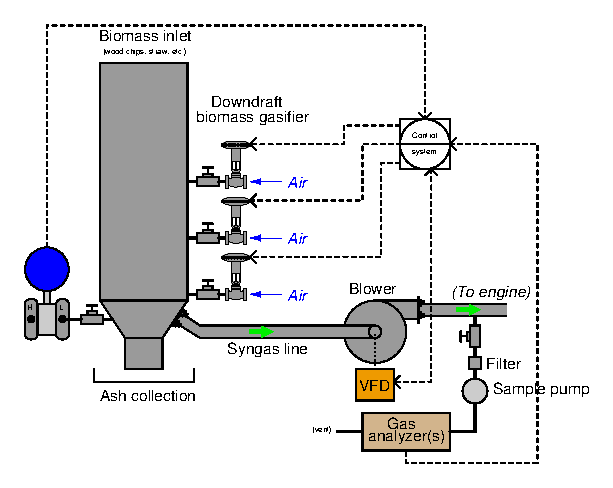
\includegraphics[width=15.5cm]{i01535x01.eps}$$

I tillegg til hydrogen og karbonmonoksid finnes det andre gasser i ``syngass''-utløpet fra forgasseren, som vi ønsker å måle for å kunne styre de kjemiske reaksjonene inne i forgasseren riktig. Disse inkluderer nitrogenoksid (NO) og karbondioksid (CO$_{2}$). Etter undersøkelse finner du to ulike analyseteknologier som kan måle alle disse gassene nøyaktig: den ene er en {\it NDIR}-analysator (ikke-dispersiv infrarød) med flere detektorer, og den andre er en {\it kromatograf}. For denne applikasjonen finner du tilfeldigvis analysatorer av begge typer til omtrent samme kostnad, noe som fjerner kostnad som avgjørende faktor ved valg av analysetype.

NDIR-analysatorer har vanligvis målemessig dødtid i størrelsesorden sekunder, mens kromatografer typisk har målemessig dødtid i størrelsesorden minutter. Basert på dette kriteriet, hvilken analyseteknologi er best egnet for lukket sløyferegulering, og viktigst av alt {\it hvorfor?}

\vskip 20pt \vbox{\hrule \hbox{\strut \vrule{} {\bf Forslag til sokratisk diskusjon} \vrule} \hrule}

\begin{itemize}
\item{} Forklar hvorfor differansetrykktransmitteren har {\it lavtrykks}-porten koblet til forgasseren (med høytrykks-porten luftet), og ikke omvendt.
\item{} Forklar hvorfor en {\it VFD} er et godt valg som sluttregulerende element på syngasslinjen, i stedet for en blåser med konstant hastighet kombinert med reguleringsventil.
\item{} Identifiser de viktigste sikkerhetsfarene i denne prosessen, samt hvilket personlig verneutstyr (PPE) operatører og teknikere kan bruke når de arbeider i nærheten.
\end{itemize}

\underbar{file i01535}
%(END_QUESTION)





%(BEGIN_ANSWER)

NDIR-analysatoren er klart det beste valget når vi vurderer dødtid. Mer dødtid i en tilbakekoblet sløyfe gir tregere (mulig) automatisk reguleringsrespons, fordi en regulatorrespons som er passende for en sløyfe med minimal dødtid vil oscillere når ekstra dødtid er til stede.

For en mer fullstendig forklaring, se {\it Lessons In Industrial Instrumentation} i seksjonen som beskriver ``dead time'' som prosessegenskap, og hvordan dette påvirker tilbakekoblet regulering.

%(END_ANSWER)





%(BEGIN_NOTES)

NDIR-analysatoren, med mindre dødtid enn en kromatograf, ville være det beste valget for lukket sløyferegulering.

\vfil \eject

\noindent
{\bf Oppsummeringsquiz:}

Forklar hvorfor {\it dødtid} er en ulempe i en tilbakekoblet reguleringssløyfe.

\begin{itemize}
\item{} Dødtid forsinker regulatorens bytte fra auto til manuell
\vskip 5pt 
\item{} Dødtid gjør oscillasjon (sykling) langt mer sannsynlig
\vskip 5pt 
\item{} Dødtid forvrenger nøyaktigheten i reguleringsventilens posisjonering
\vskip 5pt 
\item{} Dødtid forvrenger nøyaktigheten i målingen under stasjonære forhold
\vskip 5pt 
\item{} Dødtid begrenser maksimal produksjonsrate i prosessen
\vskip 5pt 
\item{} Dødtid gjør at reguleringsventilen må bevege seg mer, noe som gir for tidlig slitasje
\end{itemize}


%INDEX% Control, basics: process dead time
%INDEX% Measurement, analytical: chromatography
%INDEX% Measurement, analytical: nondispersive optical
%INDEX% Process: biomass gasification (downdraft gasifier)

%(END_NOTES)

